\documentclass[a4paper,12pt,twoside,no-math]{report} 
% Specify required margin widths and setup geometry of the thesis
\usepackage{geometry}
\geometry{
	a4paper,
	left=1.25in,
	right=1in,
	top=1in,
	bottom=1in
}
\usepackage[svgnames]{xcolor}
\usepackage{graphicx, pdfpages}
% Set path/directory where all figures are stored.
\graphicspath{ {figures/} }

%%
\usepackage{titlesec}
% Format section headings with sans-serif font
\titleformat{\section}
{\Large\bfseries\sffamily}
{\thesection}{1em}{}
% Format chapter headings with sans-serif font
\titleformat{\chapter}[display]
{\Huge\bfseries\sffamily}
{\chaptertitlename\ \thechapter}{20pt}{\Huge}

% Format subsection headings with sans-serif font
\titleformat{\subsection}
{\large\bfseries\sffamily}
{\thesubsection}{1em}{}

% Format subsubsection headings with sans-serif font
\titleformat{\subsubsection}
{\bfseries\sffamily}
{\thesubsubsection}{1em}{}

\usepackage{fancyhdr}
\usepackage{float}
\usepackage{tabularx}
\usepackage{epigraph}
\setlength{\epigraphwidth}{0.6\textwidth}
\setlength{\epigraphrule}{0pt}
%%%*********************************************
\newcommand{\myopeningquote}{%
  \raisebox{-0.4\height}{\scalebox{3}{\textcolor{Silver}{``}}~~}%
}
\newcommand{\myclosingquote}{%
  \raisebox{-0.45\height}{\scalebox{3}{\textcolor{Silver}{''}}}%
}


\usepackage[framemethod=TikZ]{mdframed}

\newenvironment{Frame}[1][]{%

    \begin{mdframed}[%
        frametitle={\textsf{#1}},
        skipabove=\baselineskip plus 2pt minus 1pt,
        skipbelow=\baselineskip plus 2pt minus 1pt,
        linewidth=0.5pt,
        frametitlerule=true,
        frametitlebackgroundcolor=Silver,
        roundcorner=10pt,
        nobreak=true
    ]%
    \rmfamily
}{%
    \end{mdframed}
}
\usepackage{amsmath, amssymb, fixmath, physics, cancel}
\usepackage[no-math]{fontspec}
\usepackage{newcomputermodern}
\usepackage[scaled=1.0]{XCharter}
\usepackage[final]{microtype}
\linespread{1.3}
%$$$$$$$
\usepackage[
	pdfauthor={Aditya Dev},
	pdftitle={},
	pdfsubject={MS19022 MS Thesis},
	pdfkeywords={},
	backref=page,
	hypertexnames=false
]{hyperref}
\renewcommand*{\backref}[1]{}
\renewcommand*{\backrefalt}[4]{{\footnotesize [%
    \ifcase #1 Not cited.%
	\or Cited on page~#2%
	\else Cited on pages #2%
	\fi%
]}}
\hypersetup{
	colorlinks = true,
	linkcolor={red!50!black},
	citecolor={blue!50!black},
	urlcolor={blue!80!black}
}
\newcommand{\refapp}[1]{Appendix~\ref{#1}}
\newcommand{\refchap}[1]{Chapter~\ref{#1}}
\newcommand{\refeq}[1]{Eqn.~\ref{#1}}
\newcommand{\reffig}[1]{Figure~\ref{#1}}
\newcommand{\refsec}[1]{Section~\ref{#1}}
\newcommand{\reftab}[1]{Table~\ref{#1}}

\renewcommand{\vec}[1]{\mathbold{#1}}
\newcommand{\mat}[1]{\mathbold{#1}}
\newcommand{\psid}{\psi ^\dagger}
\newcommand{\psibar}{\overline{\psi}}
\newcommand{\ketpsi}{\ket{\psi}}
\newcommand{\kket}[1]{\left| #1 \right\rAngle}
\newcommand{\bbra}[1]{\left\lAngle #1 \right|}
\newcommand{\ketPsi}{\kket{\Psi}}
\newcommand{\innerGlob}[2]{\left\langle #1 |  #2 \right\rAngle}
\newcommand{\oper}[1]{{\operatorname{#1}}}
\renewcommand{\H}{\oper{H}}
\newcommand{\I}{\oper{I}}
\newcommand{\Vinter}{\oper{V}}
\newcommand{\Vs}{\oper{V}_s}
\newcommand{\doubleunderbar}[1]{\underbar{\underbar{#1}}}
\begin{document}


% Use '\thispagestyle{empty}' to ensure that this page
% is not counted in page numbering.
\thispagestyle{empty}

% Set required margin widths for first few pages.
\newgeometry{top = 2.5in, left = 1.25in, right = 1in, bottom = 1in}
\begin{titlepage}

    \begin{center}
        \sffamily
        \LARGE
        \textbf{Relational Dynamics From Entangled Eigenstates}
        \vspace{1cm}
        
        \Large
        \textbf{Aditya Dev}
    
        \vspace{1cm}
        \large
        
        \textit{A dissertation submitted for the partial fulfilment of
        BS-MS dual degree in Science}
        
        \vspace{3.5cm}
    
        
\includegraphics[trim={5mm 5mm 5mm 5mm},clip,width=8cm]{HighResolutionLogo.jpg}
        \vspace{1cm}
        
        \large
        \textbf{Indian Institute of Science Education and Research, Mohali}\\
        \large
        \textbf{\today} 
    
    \end{center}
    
    
    \end{titlepage}

% Use '\thispagestyle{empty}' to ensure that this page
% is not counted in page numbering.
\thispagestyle{empty}
\cleardoublepage

% Use Roman Page Numbering for first few pages.
\pagenumbering{Roman}

{\sffamily \begin{center}
    \textbf{\Large Certificate of Examination}
\end{center}

This is to certify that the dissertation titled \textbf{Relational Quantum Dynamics From Entangled Eigenstates} submitted by 
\textbf{Aditya Dev} (Reg. No. MS19022) for the partial fulfillment of BS-MS Dual Degree 
programme of the institute, has been examined by the thesis committee duly appointed by the 
institute. The committee finds the work done by the candidate satisfactory and recommends 
that the report be accepted.

\vspace{4cm}

Dr. Abhishek Chaudhuri \hspace{0.9cm} Dr. Ambresh Shivaji \hspace{0.9cm} Dr. Ramandeep S. Johal

\vspace{4cm}

\begin{flushright}
    Dr. Abhishek Chaudhuri
    \\
    (Supervisor)
    \\
    \vspace{4cm}
    Dated: \today
\end{flushright}

\cleardoublepage

% Declaration.
\begin{center}
    \textbf{\Large Declaration}
\end{center}
The work presented in this dissertation has been carried out by me under the joint supervision of \textbf{Dr. Abhishek Chaudhuri} at the Indian Institute of Science Education and Research, Mohali, and \textbf{Prof. Dr.  Jan Micheal Rost} at Max Planck Institute for the Physics of Complex Systems, Dresden Germany. 

\vspace{0.4cm}

This work has not been submitted in part or in full for a degree, a diploma, or a fellowship to any other university or institute. Whenever contributions of others are involved, every effort is made to indicate this clearly, with due acknowledgment of collaborative research and discussions. This thesis is a bonafide record of my original work, and all sources listed within have been detailed in the bibliography.

\vspace{2cm}

\begin{flushright}
Aditya Dev
\\
(Candidate)
\\
Dated: [Enter Relevant Date]
\end{flushright}

In my capacity as the supervisor of the candidate's project work, I certify that the above statements by the candidate are true to the best of my knowledge.

\vspace{2cm}

\begin{flushright}
Dr. Abhishek Chaudhuri
\\
(Supervisor)
\\
Dated: [Enter Relevant Date]
\end{flushright}

\cleardoublepage

% Acknowledgements.
\include{acknowledgement}}
% Abstract.
%\fontfamily{ptm}\selectfont % Times font
\addcontentsline{toc}{chapter}{\textbf{Abstract}}
\begin{center}
    \textbf{\Large Abstract}
\end{center}

Use this section to include an abstract of the thesis.

\newpage
\restoregeometry

% Creates a List of All Figures.
\addcontentsline{toc}{chapter}{\textbf{List of Figures}}
\listoffigures

\newpage

% Creates a List of All Tables.
\addcontentsline{toc}{chapter}{\textbf{List of Tables}}
\listoftables

% Creates a Table of Contents.
\tableofcontents

\newpage
% Certificate of Examination.


% Use Arabic Page Numbering for the rest of the thesis.
\pagenumbering{arabic} 
% Chapter 1 - Introduction.


%%%
% This code snippet takes care of the required  
% Equation/Figure numbering scheme.
\renewcommand\thefigure{\thechapter.\arabic{figure}}    
\renewcommand{\theequation}{\thechapter.\arabic{equation}}
\setcounter{equation}{0}
\setcounter{figure}{0}
%%%
\chapter{Introduction\label{chap:introduction}}


The unification of Quantum Mechanics and General Relativity has long been
the Holy Grail of physics since their development.
Despite extensive research, no satisfactory theory has yet been
proposed to solve this challenge. General relativity states that a physical
theory should not depend on background structures.
However, conventional quantization methods often introduce background structures,
such as imposing the canonical commutation relations on constant-time hypersurface. The Hamiltonian of a
generally covariant theory, such as general relativity, is constrained to
vanish in the absence of boundaries~\cite{gielen2023quantum}. Attempts to quantize gravity using 
canonical quantization lead to a Hamiltonian constraint, the Wheeler-DeWitt equation
(i.e., \(\oper{H} \ketPsi = 0\)). This leads to an infamous problem known as
``The problem of time'' in the canonical approach to quantum gravity
[Refer to \refapp{appen:problemoftime} for more details]. The issue is that
quantum states of space-time (and matter in it) do not seem to undergo any time evolution, as
dictated by the constraints of the theory. 

In quantum cosmology, the universe is described by a wave function whose dynamics is governed by the Wheeler-DeWitt equation, the quantized Hamiltonian constraint of the system.
Due to inherent mathematical ambiguities in the Wheeler-DeWitt equation, it is often unreliable
to extend beyond the semi-classical approximation~\cite{cooke2010qcintro}. The wave function
in this approximation is provided by the WKB wave function, \(\Psi_{\mathrm{WKB}} 
\approx \exp\left[iS_0/\hbar\right]\psi(\{x_n\})\); where \(S_0\) is 
a function which obeys the classical Hamilton-Jacobi equation for the gravitational
field~\cite{gielen2023quantum}. Then we substitute this WKB analysis into the
Wheeler-DeWitt equation and applying the relevant approximations leads to the time-dependent Schr\"odinger equation.  Briggs and Rost~\cite{briggs2001derivation} 
have proposed a similar solution to the problem from an atomic and molecular
physics perspective, and their approach is discussed in~\refchap{chap:briggs_rost_semiclassic}.

On the other hand, for locally relativistic quantum field theories, it has been demonstrated
that the long-range Coulomb field causes the total ``charge'' operator to commute
with all quasi-local observables, implying a superselection rule for charges~\cite{Strocchi:1974xh} 
[Refer to \refapp{appen:superselection} for further details].
Analogously, due to the coupling of energy with the long-range gravitational field, 
there is speculation about the existence of a superselection rule for energy~\cite{page1983evolution}.
This implies that only operators that commute
with the Hamiltonian can be observable. However, such observables are stationary
(i.e., constants of motion). How can we observe time evolution if the only observables
we can observe are stationary i.e., they do not evolve at all?

The problem of time is a manifestation of background independence rather than the
``timelessness'' of quantum mechanics, and means that physical states do not evolve
relative to an external background time. Instead, time evolution must be extracted relationally, 
by selecting certain quantized degrees of freedom to serve as an internal timekeeper, 
i.e., pick some quantized degrees of freedom to serve as an internal time. 
Even in our everyday ``classical' world, we never directly measure time; instead, we measure the
position or angular displacement of a pendulum or a dial and use that measurement to \emph{define} a
unit of time. The use of relational time in Quantum
Mechanics is a framework in which one promotes all variables to quantum operators and
later chooses one of the variables to operate like a ``clock'' degree of freedom.

Apart from the semi-classical approaches employed in quantum cosmology, various other 
avenues exist to address the time problem from a purely quantum mechanical standpoint~\cite{hohn2021trinity}. 
One such approach is the ``Page-Wootters Formalism'' (abbreviated P\&W formalism), 
which defines relational dynamics in terms of conditional probabilities for the clock and 
evolving degrees of freedom~\cite{page1983evolution}. To date, no one has successfully tackled 
the problem involving general interaction potentials [with the exception of~\cite{Smith:2017pwx} 
to a certain extent]. The original formulation due to P\&W is no exception, as it also neglects 
the interaction between the environment and the system. However, recent work by Gemsheim and Rost 
has developed a relational formalism based on the P\&W formalism, which now includes the 
environment-system interaction~\cite{Gemsheim:2023izg}. This advancement provides the necessary 
tools to study relational dynamics for a general system-environment setting. Their approach is 
discussed in detail in~\refchap{chap:sebgem_Rel}.


The primary objective of this work is to study the transition from quantum mechanical approach to semi-classics, in the limit of a 
large environment\footnote{The notion of a ``large" environment will be elaborated upon
in subsequent chapters.}

\newpage

\clearpage

\newpage


\renewcommand\thefigure{\thechapter.\arabic{figure}}    
\renewcommand{\theequation}{\thechapter.\arabic{equation}}
\setcounter{equation}{0}
\setcounter{figure}{0}
%%%
\chapter[Time Emergence in Quantum-Classical Interactions
]{Emergence of Time dependence 
through interaction with a Semi-classical Environment\label{chap:briggs_rost_semiclassic}}

In modern textbooks, the Time-dependent Schr\"odinger equation (TDSE) is either introduced as a \emph{fundamental}
equation governing the time evolution of a quantum wave function, with the Time-independent Schr\"odinger
equation (TISE) as a special case, or it is derived from the correspondence with classical Hamilton-Jacobi 
theory.

Briggs and Rost~\cite{briggs2001derivation} presented an alternative derivation of the TDSE that partitions
the ``global" Hilbert space into a system and an environment. They then employed the WKB ansatz 
for the environment's wave function, effectively treating the environment semi-classically. Their analysis offers a clear physical interpretation of the time parameter, which arises from a directional gradient of the classical action along the environment trajectory.
This chapter presents the analysis by Briggs and Rost in ~\cite{briggs2001derivation}.

Consider a global system with Hamiltonian $\operatorname{H}$, which comprises a system $S$ and an environment $\mathcal{E}$. 
The TISE for this system is given by
\begin{equation}
\label{eqn:chap2_TISE}
\operatorname{H}\Psi = E\Psi, \quad \operatorname{H} = \operatorname{H}_S + \operatorname{H}_{\mathcal{E}} + \operatorname{H}_{\mathcal{SE}}.
\end{equation}
where $\operatorname{H}_S$ and $\operatorname{H}_{\mathcal{E}}$ are the Hamiltonians of the system 
and the environment respectively and $\operatorname{H}_{\mathcal{SE}}$ is the interaction
Hamiltonian between the system and the environment\footnote{$\operatorname{H}_{\mathcal{SE}}\equiv \operatorname{H}_{\mathcal{SE}}(x, R)$}.

The total wave function $\Psi$ can be written as
\begin{equation}
    \label{eqn:chap2_total_wavefunction}
    \Psi(x, R) = \sum  \psi_m (x, R) \chi_m(R).
\end{equation}
Where \(\{\psi 's\}\) represent the energy eigenstates of \(\operatorname{H}_{\mathcal{S}} + \operatorname{H}_{\mathcal{SE}}\) at a fixed $R$, with \\ \(\epsilon_n (R) =  \bra{\psi_n}\operatorname{H}_{\mathcal{S}} + \operatorname{H}_{\mathcal{SE}}\ket{\psi_n}\), and $x$ and $R$ represent the coordinates of the system and the environment, respectively.
\footnote{We have assumed that the environment is large enough so the system  has a 
no effect on the environment's states. Furthermore, \(\braket{\chi_m}{\chi_n} \not = \delta_{mn}\).}. 
The environment Hamiltonian is assumed to be of the form
\begin{equation}
    \label{eqn:chap2_env_hamiltonian}
    \operatorname{H}_{\mathcal{E}} = \operatorname{K} + \operatorname{V}_{\mathcal{E}} (R).
\end{equation}
with:
\begin{equation}
    \operatorname{K} = \frac{-\hbar^2}{2M} \sum_i \frac{\partial^2}{\partial R_i^2} = \frac{-\hbar^2}{2M} 
    \nabla _R^2.
\end{equation}

Substituting ~\refeq{eqn:chap2_total_wavefunction} in ~\refeq{eqn:chap2_TISE} and projecting onto
$\psi_n(x, R)$ gives a coupled TISE for the environment wavefunction\footnote{Notice 
that, we integrate only over $x$.}~\cite{briggs2001derivation}:
\begin{equation}
    \label{eqn:briggs_rost_eq5}
    \begin{aligned}
        \sum_{m} \bra{\psi_n} \left(\frac{-\hbar^2}{2M} \nabla_R^2 \right) \ket{\psi_m} \chi_m(R) 
    + \operatorname{V}_{\mathcal{E}}(R) \chi_n(R)\\
    + \sum_{m} \bra{\psi_n} \operatorname{H}_{\mathcal{S}} + \operatorname{H}_{\mathcal{SE}}\ket{\psi_m}\chi_m(R) = E \chi_n(R).
    \end{aligned}
\end{equation}

The ``potentials'':
\begin{equation}
    \mathcal{V}_{mn}(R) = \bra{\psi_m} \operatorname{H}_{\mathcal{S}} + \operatorname{H}_{\mathcal{SE}}
    \ket{\psi_n}.
\end{equation}
depending on the state of the quantum system, provide the energy surface
which determines the dynamics of the environment. The coupling from the kinetic term is
\begin{equation}
    \begin{gathered}
        \bra{\psi_m} \left(\frac{-\hbar^2}{2M} 
        \nabla_R^2 \right) \ket{\psi_n} \chi_n(R) \\
        = -\frac{\hbar^2}{2M} \sum_k \left(\delta_{mk} \nabla_R+ \bra{\psi_m}\nabla_R
    \ket{\psi_k}\right)\left(\delta_{kn} \nabla_R+ \bra{\psi_k}\nabla_R^2\ket{\psi_n}\right)
     \chi_n(R).
    \end{gathered}
\end{equation}

We define
\begin{equation}
    \Lambda_{mn}(R) = i\hbar \bra{\psi_m}\nabla_R\ket{\psi_n}.
\end{equation}
Now, using above definitions, ~\refeq{eqn:chap2_TISE_proj} can be written as
\begin{equation}
    \label{eqn:chap2_clc_evol}
    \sum_m \left[ \frac{1}{2M} ({\hat{P}}^2)_{nm} +  
    \mathcal{V}_{nm}(R)\right] \chi_m(R) + \operatorname{V}_{\mathcal{E}}(R) \chi_n(R) 
    = E \chi_n(R).
\end{equation}

Where
\begin{equation}
    {\hat{P}}_{nm} = -i\hbar \left(\mathbb{I}\nabla_R - \frac{i}{\hbar}
    \hat{\Lambda} \right) =
 \left(\mathbb{I}P_R - \hat{\Lambda}\right) \quad \text{or} \quad P_{ij} = 
 \left(\delta_{ij}P_R - {\Lambda}_{ij}\right).
\end{equation}
Notice that the kinematic coupling
$\hat{\Lambda}$ appears as a vector potential. 

The set of equations for system wavefunction is given by
\begin{multline}
    \label{eqn:chap2_system_evol}
    \sum_{m} \chi_m(R) \left[
    \operatorname{H}_{\mathcal{S}} + \operatorname{H}_{\mathcal{SE}}(x, R)  - \left(
        E - \operatorname{V}_{\mathcal{E}}(R) + 
        \frac{1}{\chi_m} \frac{\hbar^2}{2M} \nabla_R^2 \chi_m
    \right) \right. \\\left. - \frac{\hbar^2}{2M} \nabla_R^2 - 
    \frac{\hbar^2}{M\chi_m} \nabla_R \chi_m \cdot \nabla_R \right] \psi_m(x, R) = 0.
\end{multline}

The main approximation in this derivation would be to disentangle 
~\refeq{eqn:chap2_clc_evol} and ~\refeq{eqn:chap2_system_evol}. To do so, 
we assume that the environment is large enough so that the changes in the system,
i.e. the variation in matrix elements $\mathcal{V}_{mn}$ and $\Lambda_{mn}$, have
no effect on the environment dynamics, i.e., we neglect the off-diagonal terms. 

The fist step would be to neglect in ~\refeq{eqn:chap2_clc_evol}  all the off-diagonal
matrix elements, which gives:
\begin{equation}
\label{eq:chap2_no_off_diag}
    \left[ \frac{1}{2M} \left(P_R -  
    \Lambda_{nn}(R)\right)^2 + \operatorname{V}_{\mathcal{E}} + E_n(R) \right] \chi_n(R) = E \chi_n(R).
\end{equation}
with \(E_n(R) = \mathcal{V}_{nn}(R) \). The vector potential \(\Lambda_{nn}\), since now diagonal in the above case, can be included in the
definition of an effective environment momentum operator. 

The second step would be to use a semi-classical approximation for each \(\chi_m(R)\), i.e., we write
\begin{equation}
\label{eqn:chap2_WKB_clc}
    \chi_{n}(R) = a_n(R) \exp\left(\frac{i}{\hbar} W_n(R)\right) \equiv \exp\left(\frac{i}{\hbar} W(R, E - \epsilon_n)\right) .
\end{equation}

with
\begin{equation}
    \label{eqn:chap2_clc_action}
    \nabla _R W_n = \vec{P}_n.
\end{equation}
where the classical momentum 
\(\vec{P}_n\) and position \(\vec{R}_n\) are decided by Hamilton's equations:
\begin{eqnarray}
    \label{eqn:chap2_hamilton_eqns1}
    \frac{d\vec{P}_n}{dt} &=& -\nabla_{{R}_n} H = \nabla_{R_n}\left( \operatorname{V}_{\mathcal{E}}(R) + E_n(R)\right)\\
    \label{eqn:chap2_hamilton_eqns2}
    \frac{d\vec{R}_n}{dt} &=& \nabla_{{P}_n} H.
\end{eqnarray}

For the standard kinetic energy \(\frac{\vec{P}^2}{2M}\), one obtains from 
~\refeq{eqn:chap2_hamilton_eqns2} that \(\vec{P}_n = M\frac{d\vec{R}_n}{dt}\). It is at this point
that the time parameter enters the picture. To the leading order in \(\hbar\), one can write:
\begin{equation}
    \frac{\hbar}{iM} \nabla_R \chi_n = \frac{\chi_n}{a_n} \frac{\hbar}{iM} \nabla _R a_n + 
    \chi_n \frac{1}{M} \nabla_R W_n \approx \chi_n \frac{d\vec{R}_n}{dt}.
\end{equation}
For the system \(\mathcal{S}\) the equation coupled to ~\refeq{eq:chap2_no_off_diag} now reads
\begin{equation}
    \label{eqn:chap2_system_evol_mod2}
    \sum_{m} \chi_m(R) \left[
    \operatorname{H}_{\mathcal{S}} + \operatorname{H}_{\mathcal{SE}}(x, R)  - E_m(R)  - \frac{\hbar^2}{2M}\nabla^2 _R -
    i\hbar \frac{d \vec{R}_m}{dt} \cdot \nabla_R \right] \psi_m (x, R)= 0.
\end{equation}

It has been shown~\cite{briggs2001derivation} that in the above equation,
the term \((\hbar^2/2M)\nabla^2 _R\) with higher-order gradient couplings can be neglected in comparison
with the term
\begin{equation*}
i \hbar  \frac{d \vec{R}_n}{dt} \cdot \nabla_{R} := i \hbar \dfrac{d}{d\tau_n}.
\end{equation*}
Hence, ~\refeq{eqn:chap2_system_evol_mod2} can be written as
\begin{equation}
    \label{eqn:chap2_system_evol_mod3}
    \sum_{m} \chi_m(R) \left[
    \operatorname{H}_{\mathcal{S}} + \operatorname{H}_{\mathcal{SE}}(x,
   \{ \tau_m\})  - E_m(\{\tau_m\})  - i \hbar \dfrac{\partial }{\partial \tau_m} \right] 
    \psi_m (x, R)= 0.
\end{equation}
We have replaced the quantum \(R\) dependence by a ``classical time" like dependence on \(\{\tau_m\}\).

In the approximation represented by ~\refeq{eqn:chap2_clc_action} and
~\refeq{eqn:chap2_system_evol_mod3}, the environment shows classical dynamics, but
the state of the quantum system determines its motion and, hence, the interaction time with the system. This represents the final impact of the quantum influence on the environment. This influence diminishes as the environment becomes fully disentangled
from the system, allowing it to function as an external clock that reads a unique time~\cite{briggs2001derivation}.

This simplification is achieved in the approximation when ~\refeq{eqn:chap2_WKB_clc} becomes
\begin{equation}
    \label{eqn:chap2_clc_action2}
    \chi_n(R) = a_n(R) \exp\left(\frac{i}{\hbar} W(R)\right).
\end{equation}
%if the variation of \(E_n\) in ~\refeq{eqn:chap2_hamilton_eqns1} are negligible compared to \(V_{\mathcal{E}}\) or
which is valid  in the limit \(\epsilon_n \ll E\). It is at this point that the Environment gets fully disentangled from the system. Then we get from ~\refeq{eqn:chap2_clc_action2}, a unique time derivative
\begin{equation}
    \label{eqn:chap2_clc_action3}
    \nabla_R W = M \dfrac{d \vec{R}}{dt}
\end{equation}

Also, one can eliminate \(E_m(t)\) using a purely time-dependent phase transformation and writing 
\(\psi_{\mathcal{S}}(x) = \sum_{n}a_n \psi_n(x)\), ~\refeq{eqn:chap2_system_evol_mod3} becomes:
\begin{equation}
    \label{eqn:chap2_system_evol_mod4}
     \left[
    \operatorname{H}_{\mathcal{S}} + \operatorname{H}_{\mathcal{SE}}(x, t)- i \hbar \dfrac{\partial}{\partial t} \right] 
    \psi_m (x,t)= 0
\end{equation}

This gives the TDSE for the quantum system alone. Now, the dynamics of the environment is given by the classical equation of motion, with the system having no effect on it. However, the quantum system is affected by the environment
through the term \(\operatorname{H}_{\mathcal{SE}}\)

\newpage

\clearpage

\newpage
\renewcommand\thefigure{\thechapter.\arabic{figure}}    
\renewcommand{\theequation}{\thechapter.\arabic{equation}}
\setcounter{equation}{0}
\setcounter{figure}{0}
%%%
\chapter[Quantum Relational Dynamics for Interacting Quantum Systems]{Relational Quantum Mechanics: With System and Environment Interaction\label{chap:sebgem_Rel}}



We start by \emph{reformulating} the time independent Schr\"odinger equation as an \emph{invariance principle}~\cite{Gemsheim:2023izg}
\begin{equation}
    \label{eq:invariance_principle}
        \exp\left[i\lambda(\H - E\I)\right] \ketPsi = \ketPsi. 
\end{equation}
Where  \(\lambda\) is any complex-valued parameter, $\H$ is the Hamiltonian of the global system, and \(\ketPsi\) is the global state vector. Differentiating (\refeq{eq:invariance_principle}) with respect to \(\lambda\) one gets  the usual Time Independent Schr\"odinger Equation (TISE)
\begin{equation*}
    \H \ketPsi = E \ketPsi.
\end{equation*}

For our analysis, we assume that λ is real. We partition the total Hilbert space $\mathcal{H}$ into two components to extract the dynamics. A system \(\mathcal{H}_s\) and a clock \(\mathcal{H}_c\). We re-write 
\begin{equation}
    \H = \H_s \otimes \I_c + \I_s \otimes \H_c + \Vinter .
\end{equation}

Since the system and environment\footnote{Please note that the words `clock' and `environment' will be used synonymous. The term ``system" denotes a subsystem (excluding the environment) of a global Hilbert space unless otherwise specified.} are embedded in the global Hilbert space, one can single
out the system state by projecting the global state partially onto a static state of the environment. 

\paragraph{For non-interacting system and environment:} Let \(\ket{\chi}\) be a state vector 
in clock Hilbert space. 

We choose some state \(\ket{\chi_0} \in \mathcal{H_c}\). If one projects the state vector \(\ket{\chi_0}\) onto the invariance equation~(\refeq{eq:invariance_principle}) (assuming the absence of interaction, represented by \(\Vinter = \oper{0})\), one gets
\begin{equation}
\begin{gathered}
\bra{\chi_0}e^{i\lambda(\H - E)}\ketPsi = \innerGlob{\chi_0}{\Psi}\\
\bra{\chi_0}e^{i\lambda(\H_c - E)}\ketPsi =e^{-i\lambda \H_s}  \innerGlob{\chi_0}{\Psi}.
\end{gathered}
\end{equation}
We define
\begin{equation}
   \ket{\chi_\lambda} = e^{-i\lambda(\H_c - E)}\ket{\chi_0}.
\end{equation}

By conditioning the global state \(\ketPsi\) onto a clock state \(\ket{\chi_\lambda}\),
we utilize the state \(\ket{\chi_\lambda}\) as a label to associate the system state with the particular value of \(\lambda\), i.e., 
\begin{equation}
    \ket{\varphi(\lambda)}_s \equiv \innerGlob{\chi_\lambda}{\Psi}.
\end{equation}
So, 
\begin{equation}
\label{eq:nonint_sys_evol}
    \ket{\varphi(\lambda)}_s = e^{-i\lambda \H_s} \innerGlob{\chi_0}{\Psi} \equiv e^{-i\lambda \H_s}\ket{\varphi(0)}_s.
\end{equation}

Notice that the choice of \(\ket{\chi_0}\) fixes the system's initial state.
Since, \(\lambda\) in (\refeq{eq:nonint_sys_evol}) is assumed to be a continuous 
 parameter, the above equation can be interpreted as a solution to the differential equation
\begin{equation}
    i \dfrac{d}{d\lambda} \ket{\varphi(\lambda)}_s = \H_s \ket{\varphi(\lambda)}_s.
\end{equation}
Which is equivalent to (Time-dependent Schr\"odinger Equation) TDSE in units 
\(\hbar = 1\). It is crucial for the system and the environment within the global Hilbert space to exhibit entanglement. Otherwise, the system and the environment would uphold separate ``global" invariance principles, each with its own parameter, \(\lambda_s\) and \(\lambda_c\), respectively. This would leave the relationship between \(\lambda_s\) and \(\lambda_c\) unresolved~\cite{Gemsheim:2023izg}.

\paragraph{Role of parameter \(\lambda\):} The variable \(\lambda\) introduced 
in the above derivation has no physical significance. It only serves as a parameter
to track the evolution of our system. Any reparametrization of \(\lambda \to t(\lambda)\) 
has no change in the equation of the system state evolution. One can, in principle 
\footnote{As one does it always. We never measure time directly; rather, we measure
the angular position of a clock dial or the no of transition electrons made in a cesium atom.}
 parameterize the evolution using an observable of our environment 
 \(\operatorname{A}_c(\lambda)\equiv \bra{\chi_\lambda}\oper{A}_c\ket{\chi_\lambda}\). 
 An ideal choice would be to use such a $\oper{A}_c$ for which the relation between $\lambda $ and $\operatorname{A}_c$ is simple, for example, linear.

High-resolution clock states $\ket{\chi_\lambda} \propto \sum_k a_k \exp (-i\lambda E_c ^k)\ket{E_c}_k$ require a broad distribution over the clock energy eigenstates, ideally with uniform coefficients ($a_k$)\\\cite{Gemsheim:2023izg, Smith:2017pwx}. This condition is readily met when the clock's physical dimensions exceed those of the system.


\paragraph{For interacting system and environment:} So far in our analysis, we have assumed 
no interaction, i.e., \(\Vinter = \oper{0}\). However, in real scenarios, one always has some
interaction within components of a global closed system. To extend the derivation to 
non-zero \(\Vinter\), we modify our clock state as
\begin{equation}
   \begin{gathered}
      \ket{\chi_\lambda} = e^{-i\lambda(\H_c - E)}\ket{\chi_0} \to \\\ket{\chi_\lambda}
       = e^{-iS(\lambda)}e^{-i\lambda(\H_c - E)}\ket{\chi_0}
   \end{gathered}
\end{equation}
where \(S(\lambda) = \int^{\lambda}\xi(\tilde{\lambda} ) d\tilde{\lambda}\) is an extra factor introduced for 
simplifying upcoming derivations. When  projected onto this, the global state can be written as
\begin{equation}
\label{eq:TISE_undecomposed}
    \left(-\H_s + \xi(\lambda) + i\dfrac{d}{d\lambda}\right) 
    \innerGlob{\chi_\lambda}{\Psi} = \bra{\chi_\lambda}\Vinter\ketPsi.
\end{equation}
We can rearrange the above equation to write it as
\begin{equation}
\label{eq:TISE_undecomposed_simp}
    \begin{gathered}
         i\dfrac{d}{d\lambda}\innerGlob{\chi_\lambda}{\Psi} =
          \H_s\innerGlob{\chi_\lambda}{\Psi} - \xi(\lambda)\innerGlob{\chi_\lambda}{\Psi}  + \bra{\chi_\lambda}\Vinter\ketPsi.
    \end{gathered}
\end{equation}

We now decompose $\bra{\chi_\lambda}\Vinter\ketPsi$ into a Hermitian potential and a c-number. To facilitate the decomposition, we define the following:
 \begin{equation}
     \begin{gathered}
         \oper{P}_\Psi =\kket{\Psi} \bbra{\Psi}, \quad \oper{P}_\chi = \I_s \otimes \ket{\chi_\lambda}\bra{\chi_\lambda}\\
         \oper{P}_{\Psi \chi} = \oper{P}_\Psi\oper{P}_\chi /\mathcal{N}_\lambda
     \end{gathered}
 \end{equation}
where \(\mathcal{N}_\lambda = \bbra{\Psi}\oper{P}_\chi\ketPsi\). One observes that
\begin{equation}
\oper{P}_{\Psi \chi}\ketPsi = \frac{\oper{P}_\Psi\oper{P}_\chi}{\mathcal{N}_\lambda} \ketPsi
    = \ketPsi
\end{equation}
 Using above defined operators, we decompose the 
 \begin{equation}
 \label{eq:effective_Vs}
     \begin{aligned}
         \bra{\chi_\lambda}\Vinter\ketPsi = \bra{\chi_\lambda}\Vinter\oper{P}_{\Psi \chi}\ketPsi\\
         = \left[\oper{V}_s (\lambda)- \bbra{\Psi} \oper{V}\oper{P}_\chi \ketPsi/\mathcal{N}_\lambda \right] \innerGlob{\chi_\lambda}{\Psi}
     \end{aligned}
 \end{equation}
where 
\begin{equation*}
    \Vs(\lambda) = \frac{\bra{\chi_\lambda} \left(\Vinter\oper{P}_{\Psi} + \oper{P}_{\Psi}\Vinter\right)\ket{\chi_\lambda}}{\mathcal{N}_\lambda}
\end{equation*}

Inserting (\refeq{eq:effective_Vs}) into (\refeq{eq:TISE_undecomposed_simp}) and setting \(\xi(\lambda) = -\bbra{\Psi} \oper{V}\oper{P}_\chi \ketPsi/\mathcal{N}_\lambda\) we obtain
\begin{equation}
\label{eq:chap3_sebgem_TDSE}
 \boxed{ i\dfrac{d}{d\lambda}\ket{\varphi(\lambda)}_s= \left[\H_s + \Vs (\lambda)\right]\ket{\varphi(\lambda)}_s},
\end{equation}
where we defined \(\innerGlob{\chi_\lambda}{\Psi} = \ket{\varphi(\lambda)}_s\).  The phase factor  \(S(\lambda) = \int^\lambda \xi(\tau)d\tau \) introduced helps eliminate the c-number after the decomposition of the ``effective'' potential. 

We find that the final form of the Equation is equivalent to the TDSE for the remaining sub-system (\(\mathcal{H}_s\)) of the
global Hilbert space \(\mathcal{H}\).

\section{Example: Dynamics of two interacting (1/2)-spins}

\begin{figure}[!h]
    \centering
    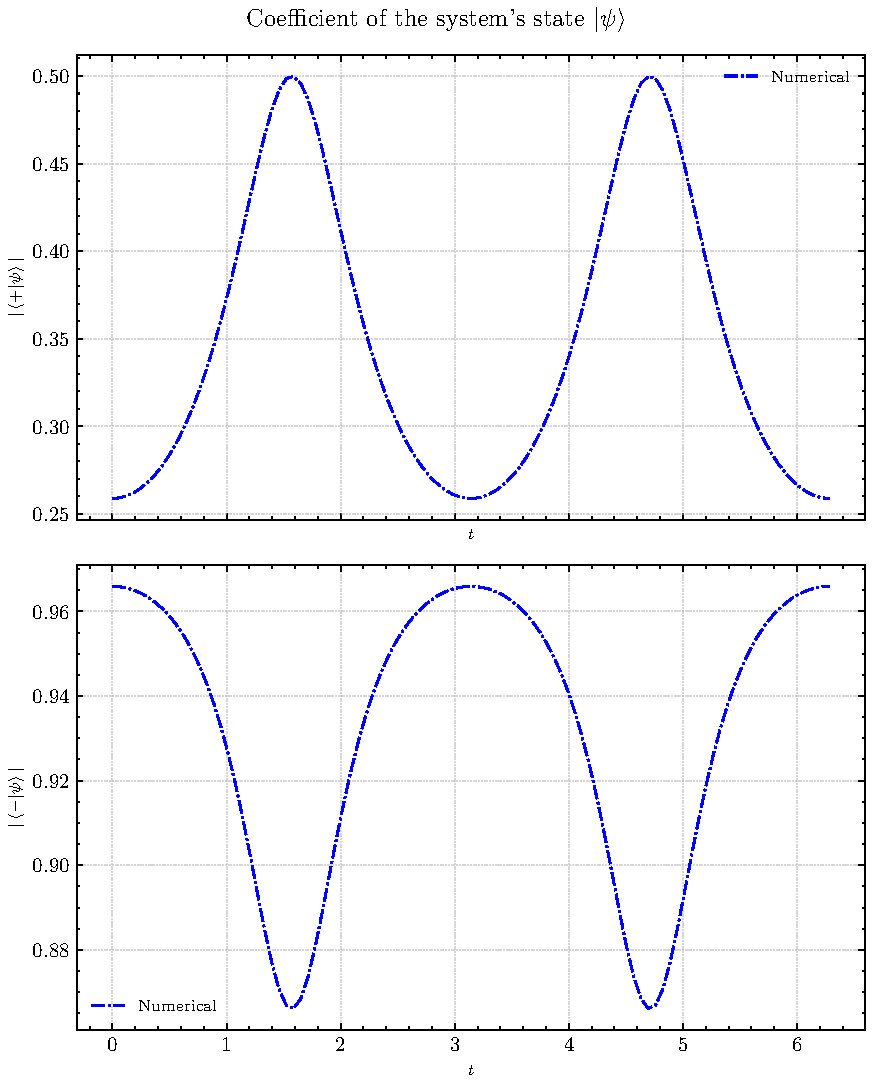
\includegraphics[]{chap3/psi_c1_c2.pdf}
    \caption{Two interacting (1/2)-spins}
    \label{fig:2spin_interact_RQM}
\end{figure}

\begin{figure}[!h]
    \centering
    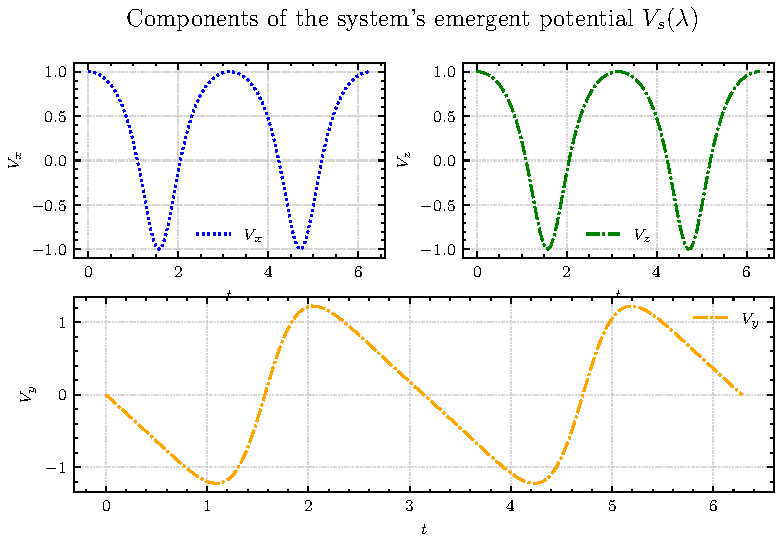
\includegraphics[width=1.0\textwidth]{chap3/Vx_Vy_Vz.pdf}
    \caption{Two interacting (1/2)-spins}
    \label{fig:2spin_emerg_pot_RQM}
\end{figure}

\newpage

\clearpage

\newpage
\renewcommand\thefigure{\thechapter.\arabic{figure}}    
\renewcommand{\theequation}{\thechapter.\arabic{equation}}
\setcounter{equation}{0}
\setcounter{figure}{0}
%%%
\chapter{Semi-Classical Relational Dynamics for Light-Matter Interaction
\label{chap:braun_briggs_jaynes}}

It has been shown in \refchap{chap:briggs_rost_semiclassic} how one can reduce a TISE 
to a TDSE for a system in the presence of a classical environment. In this chapter, 
we will discuss the application of the previous chapter to a simple model of light-matter 
interaction and enumerating the conditions that must be obtained in order to treat the 
electromagnetic field classically. The upcoming sections outlines the derivations as presented 
in~\cite{braun2004classical}. 

To get the time-dependence, we start by considerig a time-independent hamiltonian of an interacting quantum system,
with a Hamiltonian given as
\begin{equation}
    H = H_s(p, x) + H_F(P, Q) + H_I(x, Q). 
\end{equation}
where $(x, p)$ and $(Q, P)$ are (position, momentum) operator for system and boson field, respectively. 
Also, $H_s$ is the Hamiltonian of the atomic system, $H_F$ is the field hamiltonian, and $H_I$ is the interaction hamiltonian. 
The boson field hamiltonian will be takes a sum over field modes, with hamiltonian given as 
\begin{equation}
    H_F(P, Q) = \sum_{k} \frac{1}{2}\left(P_k ^2 + \omega_k^2 Q_k^2\right)
\end{equation}

We write the above Hamiltonian in terms of creating and annihilation operators
\begin{equation}
    \label{eq:class_jcm_eq1}
    H = \sum_i \epsilon_i \oper{c}^\dagger _i \oper{c}_i + \sum_k \hbar \omega_k \left(\oper{a}^\dagger _k \oper{a}_k 
    + \frac{1}{2}\right) + \hbar\sum_k  g_{jk}^k \oper{c}^\dagger _i \oper{c}_i\left(\oper{a}^\dagger _k + \oper{a}_k \right).
\end{equation}
where $c_i$ and $\oper{c}^\dagger _i$ are the annihilation and creation atomic operators for the system, 
and $a_k$ and $a^\dagger _k$ are the annihilation and creation operators for the boson field.

A special case of the above Hamiltonian is when we take a two level atom (or a spin 1/2 system)
interacting with a single mode of the electromagnetic field. \refeq{eq:class_jcm_eq1} then reduces to
\begin{eqnarray}
    \label{eq:class_jcm_eq2}
    H = \hbar \omega_0 \oper{\sigma}_z + \hbar \omega \left(\oper{a}^\dagger \oper{a} + \frac{1}{2}\right) 
    + \hbar g \oper{\sigma}_x\left(a + a^\dagger\right),
\end{eqnarray}
where $\sigma_z$ and $\sigma_x$ are the Pauli matrices. 
This special case is known as the Jaynes-Cummings model.
\section{Semiclassical Limit of the System\label{sec:class_jcm_sec1}}
As done in \refeq{eqn:chap2_total_wavefunction}, one can write in general the solution of 
TISE 
\begin{equation}
    \label{eq:class_jcm_eq2}
    (H - E)\Psi = 0
\end{equation}
with $H$ in the form of \refeq{eq:class_jcm_eq1} as 
\begin{equation}
    \label{eq:class_jcm_eq3}
    \Psi(x, Q) = \sum_{k} \chi_k(Q) \phi_k(x, Q).
\end{equation}

We employ this particular form, wherein $\chi_k(Q)$ displays no reliance on $x$, 
under the assumption that the system exerts minimal back-reaction on the field.
This assumption has been utilized previously in \refchap{chap:briggs_rost_semiclassic} 
and will be employed again in forthcoming derivations.

Doing the same exercise as in \refeq{eqn:briggs_rost_eq5}, we substitute
\refeq{eq:class_jcm_eq3} into \refeq{eq:class_jcm_eq2} and obtain a set of coupled equations

\begin{align}
    \label{eq:class_jcm_eq4}
   \sum_i \chi_i(Q) \left[H_s + H_I - \left(E - \sum_k
    \frac{1}{2}\omega_k^2 Q_k^2 + \frac{\hbar^2}{2\chi_i}\dfrac{\partial^2}{\partial Q_k^2}
    \chi_i\right) \right]\nonumber \\
    + \sum_i \chi_i(Q) \left[
        \frac{-\hbar^2}{2}\dfrac{\partial^2}{\partial Q_k^2} - 
        \frac{-\hbar^2}{\chi_i}\dfrac{\partial}{\partial Q_k}\chi_i\dfrac{\partial}{\partial Q_k}
    \right]\phi_i (x, Q) = 0.
\end{align}

\refeq{eq:class_jcm_eq4} when projected onto state \(\phi_j\) gives
\begin{align}
    \label{eq:class_jcm_eq5}
    \sum_k \left[-\frac{\hbar^2}{2}\dfrac{\partial^2}{\partial Q_k^2}
     + \frac{1}{2} \omega_k^2 Q_k^2 \right]\chi_j
    + \sum_i \bra{\phi_j}H_s + H_I\ket{\phi_i}\chi_i \nonumber \\
   - \sum_{i, k} \left[
    \bra{\phi_j}\frac{\hbar^2 \partial^2}{2 \partial Q_k^2}\ket{\phi_i}
    + \bra{\phi_j}{\hbar^2}\dfrac{\partial}{\partial Q_k}\ket{\phi_i}\dfrac{\partial}{\partial Q_k}
   \right]\chi_i = E \chi_j.
\end{align}

The equation above describes the ``close-coupled" form for \(\chi_j\). 
The off-diagonal terms account for changes in the state of the boson
field caused by changes in the system's state. Neglecting these 
off-diagonal coupling terms simplifies the equation, providing 
the state of \(\chi_j\) when the system is in state \(\phi_j\), i.e., 
\begin{equation}
    \begin{aligned}
        \label{eq:class_jcm_eq6}
    \left[\sum_k \left(-\frac{\hbar^2}{2}\dfrac{\partial^2}{\partial Q_k^2}
    + \frac{1}{2} \omega_k^2 Q_k^2\right)
    + E_j(Q) - E \right]\chi_j \\
    = \hbar^2 \sum_k \bra*{\phi_j}H_s + H_I \ket*{\phi_j}\dfrac{\partial}{\partial Q_k}\chi_j.
    \end{aligned}
\end{equation}
with 
\begin{eqnarray}
    E_j(Q) = \bra*{\phi_j}H_s + H_I - \sum_k \frac{\hbar^2}{2} \dfrac{\partial^2}{\partial Q_k^2} \ket*{\phi_i}.
\end{eqnarray}
The diagonal \(\bra*{\phi_j}H_s + H_I \ket*{\phi_j}\) terms on the RHS of \refeq{eq:class_jcm_eq6}
are zero for real \(\phi_j\) or else can be eliminated by a (Berry) phase transformation~\cite{braun2004classical}.
In addition, since we are neglecting the first order derivatives w.r.t. $Q_k$, it's consistent to neglect
the second order derivatives as well, which gives us the following equation
\begin{equation}
    \label{eq:class_jcm_eq7}
    \left[\sum_k \left(-\frac{\hbar^2}{2}\dfrac{\partial^2}{\partial Q_k^2}
    + \frac{1}{2} \omega_k^2 Q_k^2\right)
    + E_j(Q) - E \right]\chi_j (Q)= 0.
\end{equation}
this is the defining equation for the state of the boson field when the system is in state \(\phi_j\).

For, complete independence of the field from the system, we need to replace 
\(E_j(Q)\) by some fixed average energy \(\bar{E}(Q)\) and corresponding 
\(\chi_j(Q)\) by some ``mean''-field state \({\chi}(Q)\). Hence, we replace 
\begin{equation}
    \label{eq:class_jcm_eq8}
    \chi_j(Q) = a_j(Q) \chi(Q).
\end{equation}
where we assume \(a_j(Q)\) to be slowly varying function of \(Q\). The \refeq{eq:class_jcm_eq3}
reduces to
\begin{align}
    \label{eq:class_jcm_eq9}
    \Psi(x, Q) = \chi(Q) \sum_j a_j(Q) \phi_j(x) \nonumber \\
    \Psi(x, Q) =  \chi(Q)  \psi(x, Q).
\end{align}
We've identified the key approximations needed to express the exact wave function 
(\refeq{eq:class_jcm_eq3}) in the simpler, factorized form (\refeq{eq:class_jcm_eq9}). 
This step is critical because it assumes the influence of the atom on the field is minimal, while the 
field has a strong influence on the atom. Now, we can focus on deriving the effective 
Schrödinger equation for the wave function (denoted by \(\psi\)) representing the quantum system.

Note that, one can in general, view \refeq{eq:class_jcm_eq9} as a general ansatz for the wave function
and find from \refeq{eq:class_jcm_eq2}\footnote{Here we assumed only single mode of E.M field} 
\begin{align}
    \label{eq:class_jcm_eqA}
    (H - E) \Psi = \chi(Q)\left[H_S+H_I(x, Q)-\frac{\hbar^2}{2}\left(\frac{\partial^2}{\partial Q^2}\right.\right.
    & \left.\left. 
    +2 \frac{\chi^{\prime}(Q)}{\chi(Q)} \frac{\partial}{\partial Q}\right)\right] 
    \psi(x, Q) \nonumber \\
    +\psi(x, Q)\left[-\frac{\hbar^2}{2} \frac{\partial^2}{\partial Q^2}+\frac{\omega^2}{2} Q^2
    - E\right] \chi(Q) = 0
\end{align}
To streamline our analysis, we'll now focus on a single field mode. This derivation takes a 
slightly different approach compared to both the method outlined in 
\refchap{chap:briggs_rost_semiclassic} 
and the one we'll use later for the Jaynes-Cummings model (our toy model universe). 
We present this alternative approach to lay the groundwork for the new considerations 
in the next section, which will leverage coherent states.

We split the action of the total Hamiltonian on the field ad quantum system such that the 
wave function \(\chi(Q)\) described the field with energy close to total energy \(E\), while 
the reaming part of the equation describes the quantum system (with negligible energy in camparison).
Completely ignoring the influence of the quantum system on the field (back coupling) is analogous 
to neglecting the terms \(\bar{E}(Q)\) in the equations. This simplification allows us 
to select a wave function for the field, which will ultimately be treated classically. 
This is equivalet to neglecting \(\bar{E}(Q)\) and allows one to choose the wave function of the
field which is to become classical, This wave function must be an eigenstate of the fixed-field Schrödinger equation
, i.e.
\begin{equation}
    \label{eq:class_jcm_eq10}
    \left[\sum_k \left(-\frac{\hbar^2}{2}\dfrac{\partial^2}{\partial Q_k^2}
    + \frac{1}{2} \omega_k^2 Q_k^2\right)
    - E \right]\chi(Q) = 0.
\end{equation}
Under the assumption of these large (classical) energies and assuming we're sufficiently far from any 
classical turning points, we can approximate the actual wave function, denoted by $\chi(Q)$,
 by its WKB approximation, i.e., 
 \begin{equation}
    \label{eq:class_jcm_eq11}
    \chi(Q) = \exp\left(\frac{i}{\hbar}\int ^Q dQ' P(Q')\right).
 \end{equation}
where \(P(Q)\) is the momentum of the field, given as 
\begin{equation}
    \label{eq:class_jcm_eq12}
    P(Q) = \sqrt{2\left(E - \frac{1}{2}\omega^2 Q^2\right)}.
\end{equation}
Using \refeq{eq:class_jcm_eqA} - \refeq{eq:class_jcm_eq11} gives
\begin{eqnarray}
    \label{eq:class_jcm_eq13}
    \left[\sum_k \left(-\frac{\hbar^2}{2}\dfrac{\partial^2}{\partial Q_k^2}
    + \frac{1}{2} \omega_k^2 Q_k^2\right)
    - E \right]\exp\left(\frac{i}{\hbar}\int ^Q dQ' P(Q')\right) = 0 \nonumber \\
    \left[
        H_s + H_I(x, Q) - \frac{\hbar^2}{2} \dfrac{\partial^2}{\partial Q^2}
    - i\hbar P(Q) \dfrac{\partial}{\partial Q}\right] \psi(x, Q) = 0. 
\end{eqnarray}

The above differential equation describes the dynamics of (atomic part) 
the quantum system. We simplfy this equation by replacing the equation by a parameter $t$, 
which parametrizes $Q(t)$ trajectory and define
\begin{equation}
    \label{eq:class_jcm_eq14}
    P(Q)\dfrac{\partial}{\partial Q} \equiv \dfrac{\partial }{\partial t}
\end{equation}
It's evident that $P(Q)$ derived from \refeq{eq:class_jcm_eq12} corresponds to the velocity 
$\dot{Q}$, as dictated by classical equations of motion. These equations state that
$\dot{Q} = P$ and $\ddot{P} = -\omega^2 Q$, where $Q(t) = Q_0 \cos(\omega t)$ represents 
\textit{the solution, demonstrating that the parameter $t$ signifies classical time.}

We define \(\psi(x, t) = \psi(x, Q(t))\) and find from \refeq{eq:class_jcm_eq13}
\begin{equation}
    \label{eq:class_jcm_eq15}
    i \frac{\partial}{\partial t}\psi(x, t) = \left[ H_s + H_I(x,Q(t)) 
    \frac{\hbar^2}{2} \left(\frac{\ddot{Q}(t)}{\dot{Q}^3(t)}\frac{\partial}{\partial t}
    - \frac{1}{\dot{Q}^2(t)} 
    \frac{\partial^2}{\partial t^2}\right)\right]\psi(x, t).
\end{equation}

The derivatives appearing on the right-hand side stem from the second-order derivative 
$\frac{\partial^2}{\partial Q^2}$ wrt position, when expressed in terms 
of time derivatives. In the scenario of a substantial (``classical") amount of 
energy $E$, predominantly residing in the classical degree of freedom $Q$, these additional 
terms become negligible, as we will soon illustrate. Initially, it's worth noting that 
$\frac{\partial}{\partial t}$ is of the order of energy of the quantum system, 
$E_s = \langle H_s + H_I\rangle$, implying it is considerably smaller than $E$. This allows us to 
disregard the supplementary derivative terms on the right side of \refeq{eq:class_jcm_eq15}. 
Proceeding with self-consistency, and leveraging ${\dot{Q}} = P \approx \sqrt{E}$ 
for the harmonic oscillator away from its turning points, as well as 
$\ddot{Q} \approx \omega \dot{Q}$, we can estimate their respective orders of magnitude.
First, 
\begin{equation}
    \label{eq:class_jcm_eq16}
    \left \langle \frac{\hbar^2}{2} \frac{\ddot{Q}(t)}{\dot{Q}^3(t)}\frac{\partial}{\partial t} \right\rangle
    \approx E_s \frac{\hbar \omega}{E}, \text{ and } \left \langle\frac{\hbar^2}{2} \frac{1}{\dot{Q}^2(t)} 
    \frac{\partial^2}{\partial t^2} \right\rangle \approx \frac{E_s^2}{E^2}.
\end{equation}
The additional derivative terms on the right-hand side of \refeq{eq:class_jcm_eq15} 
exhibit an order of magnitude of $E_s\left(\frac{E_s + \hbar \omega}{E}\right)$. 
Hence, in comparison to the remaining terms on the right-hand side, which are of 
the order $E_s$, these additional terms are diminished by a factor approximately 
$\frac{\hbar \omega}{E} \approx \frac{1}{n}$, where $n$ represents the number of
photons in the field mode.
This factor is significantly small for a classical field. Hence, we can neglet these 
terms and write
\begin{equation}
    \label{eq:class_jcm_eq17}
    i \frac{\partial}{\partial t}\psi(x, t) = \left[ H_s + H_I(x,Q(t))\right]\psi(x, t)
\end{equation}
which is the usual form of TDSE for the quantum system interacting with the classical field.

The derivation relies on the Time-Independent Schrödinger Equation (TISE) for both the 
atom and the field. Time arises as a consequence of classical motion, serving solely as 
a derived classical parameter. It's important to note that 
the aforementioned arguments hold true only away from turning points where 
the velocity ${\dot{Q}}(t)$ is non-zero. But it's evident that the Time-Dependent 
Schrödinger Equation (TDSE) of (\refeq{eq:class_jcm_eq17}) remains valid for all times. 
The reason behind this limitation is apparent: it lies in the selection of $Q$, 
the position representation, for the field mode. 
While this choice aids in diagonalizing the coupling Hamiltonian $H_I$, 
in this representation, the real field quadrature $Q(t)$ undergoes 
harmonic motion with periodic zeros in its time derivative $Q^{\dot{}}(t)$. 
Consequently, the position representation fails to offer a global notion of time. 
Next section will illustrates how this limitation can be addressed by utilizing 
a coherent state representation of the field state.

\section{Coherent State Derivation of TDSE}
In quantum optics, coherent states hold a special place. Representing minimal uncertainty 
in both position $(Q)$ and momentum $(P)$ of the field mode, these states exhibit classical 
behavior. It's therefore unsurprising that coherent states play a crucial role in deriving 
a time-dependent Schrödinger equation for the quantum system's degrees of freedom. This 
derivation leverages a time-independent Schrödinger equation encompassing both the coupled 
quantum system and the field mode. 

We begin by writing  the total hamiltonian for single mode of E.M field in term of usual 
creation and annihilation operators as
\begin{equation}
    \label{eq:class_jcm_eq18}
    \begin{aligned}
        \H_F = \hbar \omega \left(\oper{a}^\dagger \oper{a} + 1/2\right), \\
        \H_I = \hbar \oper{S} (\oper{a} + \oper{a}^\dagger)
    \end{aligned}
\end{equation}
with \(\oper{S} = \sum_{ij}^k g_{ij} \oper{c}_i^\dagger \oper{c}_i\) as in \refeq{eq:class_jcm_eq1}.

Coherent state, defined as, \(\ket{\alpha} = \exp\left(\abs*{\alpha}^2/2 + \alpha \oper{a}^\dagger\right) \ket{0}\)
where \(\alpha\) is a complex number, is an eigenstate of the annihilation operator, i.e., 
\(\oper{a}\ket{\alpha} = \alpha \ket{\alpha}\). Some crucial properties that will be of use to us are 
\begin{equation}
    \label{eq:class_jcm_eq19}
    \begin{aligned}
        \bra*{\alpha}\oper{a}^\dagger = \alpha^* \bra*{\alpha},\\
        \bra*{\alpha}\oper{a} = \left(\dfrac{\partial}{\partial \alpha^*} + \frac{\alpha}{2}\right)\bra*{\alpha}.
    \end{aligned}
\end{equation}

Coherent states form an overcomplete basis, i.e., any state \(\ket{\psi}\) can be expanded as
\begin{equation}
    \label{eq:class_jcm_eq20}
    \ket{\psi} = \int \frac{d^2\alpha}{\pi} \ket{\alpha}\bra*{\alpha}\ket{\psi} \equiv 
    \int \frac{d^2\alpha}{\pi} \ket{\alpha}\Tilde{\chi}(\alpha, \alpha^*).
\end{equation}

where \(\Tilde{\chi}(\alpha, \alpha^*) = \bra*{\alpha}\ket{\psi}\). Note that we can 
always write  
\[\Tilde{\chi}(\alpha, \alpha^*) = \chi(\alpha^*)\exp\left(-\abs*{\alpha}/2\right)\]
where \(\chi(\alpha, \alpha^*)\) is a complex function of \(\alpha\). Instead of utilizing the position
$Q$ representation as previously done, we leverage the properties of coherent states mentioned 
above to express the Time-Independent Schrödinger Equation (TISE) within the coherent state 
representation relative to the classical degree of freedom. We write the total wave function
\begin{equation}
    \label{eq:class_jcm_eq21}
    \braket*{\alpha}{\Psi} = \exp\left(-\abs*{\alpha}^2/2\right)\chi(\alpha^*)\psi(\alpha^*).
\end{equation}
As before, we will consider \( \exp\left(-\abs*{\alpha}^2/2\right)\chi(\alpha^*)\) to 
describe the classical degree of freedom, while \(\psi(\alpha^*)\) will represent the 
quantum system without backreaction to the classical degree of freedom.

Another important property of the conherent state is it's overlap with the  photon number state, 
which is given as \( \braket*{n}{\alpha} = \exp\left(-\abs*{\alpha}/2\right) (\alpha^*)^n/\sqrt{n!} \). 
In the limit of large photon number \(n\), it's easy to see that only those coherent states 
\(\ket{\alpha}\) with 
\begin{equation}
    \label{eq:class_jcm_eq22}
    \abs*{\alpha}^2 = n
\end{equation}
will contribute significantly to the number state \(\ket{n}\).


Another significant property of coherent states is their overlap with photon number states, expressed as 
\( \braket*{n}{\alpha} = \exp\left(-\abs*{\alpha}/2\right) (\alpha^*)^n/\sqrt{n!} \). 
When considering a large photon number $n$, it becomes evident that only coherent states 
$\ket{\alpha}$ satisfying the condition:
\begin{equation}
\label{eq:class_jcm_eq22}
\abs*{\alpha}^2 = n
\end{equation}
contribute significantly to the corresponding number state \(\ket{n}\). 
With \refeq{eq:class_jcm_eq21} in mind, the TISE with $H_F$ and $H_I$ from 
\refeq{eq:class_jcm_eq20} now reads
\begin{eqnarray}
    \label{eq:class_jcm_eq23}
    \bra*{\alpha}(H - E)\ket*{\Psi} = \chi(\alpha^*)
    \left[H_s + \hbar g \left(\alpha ^* + 
    \frac{\chi'(\alpha^*)}{\chi(\alpha^*)} + \dfrac{\partial}{\partial \alpha^*}
    \right)\sigma_x + \hbar \omega \alpha^* \dfrac{\partial}{\partial \alpha^*}\right] 
    \ket*{\psi(\alpha^*)} \nonumber \\
    + \ket*{\psi(\alpha^*)}
    \left[\hbar \omega \left(
        \alpha^* \dfrac{\partial}{\partial \alpha^*} + \frac{1}{2}\right) - E\right]\chi(\alpha^*) = 0. \quad \qquad
\end{eqnarray}

The above equation corresponds to \refeq{eq:class_jcm_eqA} of position space approach. 
Just as we did in \refsec{sec:class_jcm_sec1}, we chose \(\chi\) to be an eigenstate of the field 
Hamiltonian, i.e., to be a number state \(\ket*{n}\) with energy \(E = \hbar \omega \left[n + 1/2\right]\).
In coherent state representation, 
\begin{eqnarray}
    \label{eq:class_jcm_eq24}
    \chi(\alpha^*) =  (\alpha^*)^n/\sqrt{n!}. 
\end{eqnarray}

This ensures that the second part of \refeq{eq:class_jcm_eq23} dissappears and one notices that
\begin{eqnarray}
    \label{eq:class_jcm_eq25}   
    \frac{\chi'(\alpha^*)}{\chi(\alpha^*)} = \frac{n}{\alpha^*} = \frac{\alpha^*\alpha}{\alpha^*} = \alpha.
\end{eqnarray}

Using \refeq{eq:class_jcm_eq24} and \refeq{eq:class_jcm_eq25} in \refeq{eq:class_jcm_eq23} gives
\begin{equation}
    \label{eq:class_jcm_eq26}
    \left[H_s + \hbar S \left(\alpha^* + \alpha + 
    \dfrac{\partial}{\partial  \alpha^*}\right) 
    + \hbar \omega \alpha^* \dfrac{\partial}{\partial \alpha^*} \right] \ket*{\psi(\alpha^*)} = 0.
\end{equation}
We now introduce a new parameter \(t\), which replaces \(\alpha\) analogous to what we did 
in position space representation. The parameter \(t\) is defined through a complex trajectory 
\(\alpha^*(t)\) for the coherent state field amplitude, such that 
\begin{equation}
    \label{eq:class_jcm_eq27}
    \hbar \omega \alpha^* \dfrac{\partial}{\partial \alpha^*} \equiv 
    -i \hbar\dfrac{\partial}{\partial t}.
 \end{equation}
Hence, time is determined by the classical motion of the field amplitude, which in this case is 
\begin{equation}
    \label{eq:class_jcm_eq28}
    \alpha(t) = \alpha_0 e^{-i\omega t}.
\end{equation}

Importantly, whereas the position space expression (\refeq{eq:class_jcm_eq14}) becomes 
problematic near classical turning 
points due to $P(Q) = 0$, the coherent state expression (\refeq{eq:class_jcm_eq27}) maintains finiteness throughout all times. 
Furthermore, it's noteworthy that the coherent state equation (\refeq{eq:class_jcm_eq26}) exclusively involves first-order 
derivatives. This characteristic closely resembles the first-order time-dependent Schrödinger 
equation, whereas the position space expression (\refeq{eq:class_jcm_eq15}) is of second order.

We see that the field part of the interaction Hamiltonian becomes, 
\begin{eqnarray}
    \label{eq:class_jcm_eq29}
    \left[\alpha^* + \alpha - \alpha \left(\hbar \omega \abs*{\alpha}^2\right)^{-1}
    \left(i \hbar \partial / \partial t\right) \right]
\end{eqnarray}

In large photon number limit \(1/\abs*{\alpha}^2 \approx 1/n\), vanishes. This can be 
compared to the similar discussion after \refeq{eq:class_jcm_eq15}. Therefore we find that, in 
the limit of large photon number, the TDSE for state \(\ket*{\psi(t)}\) is 
\begin{mdframed}
    \begin{equation}
        \label{eq:class_jcm_eq30}
        i\hbar \dfrac{\partial}{\partial t} \ket*{\psi(t)} = \left[
            H_s +  \hbar S \left(\alpha_0 e^{-i \omega t} + \alpha_0 e^{i \omega t}\right) 
        \right] \ket*{\psi(t)}.
    \end{equation}
\end{mdframed}

Under the assumption of a valid two-level approximation, the system can be represented 
by the operator $S = g\sigma_x$.  Crucially, unlike the equivalent result obtained in 
position space representation, the derivation of \refeq{eq:class_jcm_eq30} using coherent 
states is valid for all times.

Furthermore, this equation for a two-level system interacting with a single electromagnetic 
field mode is of critical importance. We will leverage it to compare the system's dynamics 
obtained through this approach to those obtained from a fully quantum relational dynamics 
approach in the next section.

\clearpage

\newpage



\renewcommand\thefigure{\thechapter.\arabic{figure}}    
\renewcommand{\theequation}{\thechapter.\arabic{equation}}
\setcounter{equation}{0}
\setcounter{figure}{0}
%%%

\appendix


\chapter{The Problem of Time\label{appen:problemoftime}}

In physics, the action principle is a powerful approach for formulating laws, including general relativity, which essentially describes how a system's properties change with different paths it might take. Interestingly, certain continuous transformations on variables that don't alter this action hold a hidden key.  
The significance of continuous symmetries lies in their ability to create conservation laws, as per the well-known ``Noether's Theorem''. Given the essential role of conservation laws in physics, it is both meaningful and beneficial to explore the symmetries of the action.

It is useful to distinguish between two types of symmetries: 
\begin{itemize}
\item \emph{Dynamical symmetries} corresponding to some inherent property of matter or spacetime evolution (e.g., the
Lagrangian being independent of a coordinate, leading to a conserved conjugate momentum) 
\item \emph{Non-Dynamical symmetries} arise because of the way in which we formulate
the action (e.g., the gauge symmetries). Dynamical symmetries constrain the solutions
of the equations of motion, while non-dynamical symmetries give rise to special laws
called identities. They are distinct from conservation laws because they hold regardless of whether
or not one has extremized the action.
\end{itemize}

\section{Parameterization-Invariance and Hamiltonian Constrain}
Consider a system with $n$ degrees of freedom - the generalized coordinates $q_i$ - with a parameter $t$ giving the evolution of the trajectory in configuration space. We will remove the superscript
on $q_i$ when it is clear from the context. Let the action of this system be:
\begin{equation}
	\label{eq:action_t}
	\mathcal{S} = \int L_s\left(q, \frac{dq}{dt}\right)  dt
\end{equation}
Now consider a new integration parameter \(\tau\), which now parameterizes the trajectory and promotes \(t \to t(\tau)\) 
i.e to a dynamical variable.
In terms of \(\tau\) the action (\refeq{eq:action_t}) can be expressed as:
\begin{equation}
	\mathcal{S} = \int L_s\left(q, \frac{\Dot{q}}{\Dot{t}}\right)  \Dot{t} d\tau =  \int L\left(q, \Dot{q}, \Dot{t}\right)   d\tau
\end{equation}
where \(\dot{a} \equiv \dfrac{d a}{d \tau}\) and 
\(L\left(q, \Dot{q}, \Dot{t}\right) = \Dot{t}L_s\left(q, \frac{\Dot{q}}{\Dot{t}}\right)  \).
The Hamiltonian for the modified Lagrangian is then obtained by taking the Legendre
transformation w.r.t. both \(\dot{q} \text{ and } \dot{t}\)\ ~\cite{deriglazov2011reparametrization}:
\begin{equation}
	\label{eq:hamlt_L}
	\begin{gathered}
		H =  p_t \dot{t} + p_q \dot{q} - L\\
		H =  p_t \dot{t} + \dot{t} p_q (\dot{q}/\dot{t}) - \dot{t}L_s\\
		H  = \dot{t} \left(p_t + p_q q'- L_s\right)
	\end{gathered}
\end{equation}
where \(q'=\dfrac{dq}{dt}=(\dot{q}/\dot{t})\).

Let's calculate the conjugate momenta:
\begin{equation}
	\begin{gathered}
		p_q := \frac{\partial L}{\partial\dot{q}}
		= \dot{t}\frac{\partial L_s}{\partial\dot{q}}
		=\frac{\partial L_s}{\partial(\dot{q}/ \dot{t})}\\
		p_q = \frac{\partial L_s}{\partial q'}
	\end{gathered}
\end{equation}
which coincides with the momentum conjugate to $q$ defined by $L_s(q, q′)$. Hence, (\refeq{eq:hamlt_L}) get's modified as:
\begin{equation}
	\label{eq:hamil_contrain_Hs}
	H  = \dot{t} \left(p_t + H_s\right)
\end{equation}
where \(H_s = p_q q'- L_s\) i.e Hamiltonian conjugate to \(L_s\).
We have:
\begin{equation}
	\label{eq:conh_pt}
	\begin{gathered}
		p_t := \frac{\partial L}{\partial\dot{t}}\\
		p_t = L_s + \dot{t} \frac{\partial L_s(q, q')}{\partial\dot{t}}\\
		p_t = L_s + \dot{t} \left(\frac{\partial L_s(q, q')}{\partial q} \cancelto{0}{\frac{d q}{d \dot{t}}} +
		\frac{\partial L_s(q, q')}{\partial q'} \frac{d (\dot{q}/\dot{t})}{d \dot{t}}
		\right) \\
		p_t = L_s - q'p_s = - H_s
	\end{gathered}
\end{equation}
Using (\refeq{eq:conh_pt}) in (\refeq{eq:hamil_contrain_Hs}), the equation reduces to:
\begin{equation}
	\label{eq:H0}
	\boxed{H = 0}
\end{equation}
Therefore, for parameterization-invariant theory, the Hamiltonian function 
is identically zero. It is crucial to note that this \emph{derivation makes no 
assumptions about the extremality of the action or the satisfaction of the 
Euler-Lagrange equations} by the ($q$'s). Consequently, \refeq{eq:H0}
represents a non-dynamical symmetry.

Identity $H = 0$ is very different from conservation law $H = \mathrm{constant}$ arising
from a time-independent Lagrangian. The conservation law holds only for solutions of the
equations of motion; in contrast, when the action is parameterization-invariant, 
$H = 0$ holds for any trajectory. The non-dynamical symmetry, therefore, does not
constrain the motion.

%%%
% This code snippet takes care of the required  
% Equation/Figure numbering scheme.
\renewcommand\thefigure{\thechapter.\arabic{figure}}    
\renewcommand{\theequation}{\thechapter.\arabic{equation}}
\setcounter{equation}{0}
\setcounter{figure}{0}
%%%

\chapter{Super-Selection Rule\label{appen:superselection}}


In quantum theory, physically measurable quantities of a microscopic system are represented by self-adjoint operators. However, not all of the self-adjoint operators correspond to measurable quantities. The super-selection rule is a criterion to distinguish measurable self-adjoint operator from the un-measurable ones, i.e., any measurable quantity must obey the superselection rules. By contraposition, any quantity which does not obey the superselection rules cannot be measured. It should be noted that
such a statement implies that the set of (physically realizable) observables is strictly
smaller than the set of all self-adjoint operators on Hilbert space. The notion of superselection rule (henceforth abbreviated SSR) was first introduced
in 1952 by Wick, Wightman, and Wigner~\cite{Wick:1952nb} in connection with the problem of consistently assigning intrinsic parity to elementary particles.


In the context of quantum field theory, the electric current \( J^\mu  = \overline{\psi}\gamma^\mu \psi\) is defined in terms of the Dirac spinor field operator \(\psi\) for electrons. The electric current $J^\mu$ is self-adjoint and measurable. However, the operators
\begin{equation}
	\frac{1}{2}\left(\psi + \psid \right) \qquad \frac{1}{2i}\left(\psi - \psid \right)
\end{equation}
are also self-adjoint but they are not measurable even via indirect methods.




A SSR is stated as follows: There is an operator $\oper{J}$, which we call the
superselection charge. If a self-adjoint operator $\oper{A}$ represents a measurable quantity, it must
satisfy the commutativity~\cite{TanimuraSuperSelection}

\begin{equation}
	\label{eq:superselection_law}
	\comm{\oper{J}}{\oper{A}} = 0
\end{equation}

This is a SSR, which is a necessary condition for the measurability of $\oper{A}$.
The SSR can be compared with a conservation law. The conservation of
$\oper{J}$ is formulated as

\begin{equation}
	\label{eq:conservation_law}
	\comm{\oper{J}}{\oper{H}} = 0
\end{equation}
where $\oper{H}$ is the Hamiltonian $\oper{H}$ of the system. The conservation law ~(\refeq{eq:conservation_law}) requires that
$\oper{J}$ commutes with the Hamiltonian $\oper{H}$ while the superselection rule ~(\refeq{eq:superselection_law}) requires that $\oper{J}$ commutes with all of the measurable quantities. Thus, the superselection rule is a stronger requirement for $\oper{J}$ than the conservation law. It can be said that the superselection rule is an extreme form of conservation laws.

Notice that the SSR~(Eq~\refeq{eq:superselection_law}) implies that, for all  physically measurable observables $\oper{A}$ and  any eigenvector \(\ket{\psi _i}\) of $\oper{J}$ with charge $q_i$\footnote{we assume $\oper{J}$ is non degenerate}.
\begin{equation}
	\label{eq:sSSR_orthoganility}
	\begin{gathered}
		\bra{\psi_i}\oper{J}\oper{A}\ket{\psi_j} - \bra{\psi_i}\oper{A}\oper{J}\ket{\psi_j} = 0\\
		(q_i - q_j)\bra{\psi_i}\oper{A}\ket{\psi_j} = 0\\
		\bra{\psi_i}\oper{A}\ket{\psi_j} = 0 \quad (\text{for } i\not = j)
	\end{gathered}
\end{equation}
So,  if we have a quantum state in a coherent superposition of eigenstates of superselection charge $\oper{J}$ i.e. \(\ket{\psi _+} = \frac{\ket{\psi _1} + \ket{\psi_2}}{\sqrt{2}}\). One can check that:
\begin{equation}
	\begin{gathered}
		\bra{\psi_+}\oper{A}\ket{\psi_+} =  \frac{\bra{\psi_1}\oper{A}\ket{\psi_1} +  \bra{\psi_2}\oper{A}\ket{\psi_2} + \overbrace{2\mathrm{Re}[\bra{\psi_1}\oper{A}\ket{\psi_2}]}
			^{=0}
		}{2}\\
		\bra{\psi_+}\oper{A}\ket{\psi_+} =  \frac{\bra{\psi_1}\oper{A}\ket{\psi_1} +  \bra{\psi_2}\oper{A}\ket{\psi_2}}{2} = \Tr{\rho \oper{A}}
	\end{gathered}
\end{equation}
where
\begin{equation}
	\rho = \frac{\ket{\psi_1}\bra{\psi_1} + \ket{\psi_2}\bra{\psi_2}}{2}
\end{equation}
i.e. any relative phase between \(\ket{\psi_1}\) and \(\ket{\psi_2}\) is not measurable 
and that coherent superposition of \(\ket{\psi_1}\) and \(\ket{\psi_2}\) cannot be 
verified (or prepared). For an observer, the state \(\ket{\psi_+}\) will not be any 
different from a mixed state \(\rho\). 


\clearpage

\newpage

\addcontentsline{toc}{chapter}{Bibliography}
\bibliographystyle{styles/bibsty.bst}
\bibliography{refrences}



\end{document}












